\documentclass[10pt]{beamer}

\mode<presentation> {

% \usetheme{Berlin}  % Squares
\usetheme{Madrid}  % Circles & dense
% \usetheme{Frankfurt}  % Cirles

\setbeamertemplate{headline}{%
\leavevmode%
  \hbox{%
    \begin{beamercolorbox}[wd=\paperwidth,ht=2.5ex,dp=1.125ex]{palette quaternary}%
    \insertsectionnavigationhorizontal{\paperwidth}{}{\hskip0pt plus1filll}
    \end{beamercolorbox}%
  }
}

\setbeamertemplate{navigation symbols}{}  % To remove the navigation symbols from the bottom of all slides uncomment this line

% \useoutertheme{miniframes}
% \useinnertheme{circles}

}

\usepackage{graphicx}
\usepackage{booktabs}
\usepackage{fontspec}
\usepackage{xunicode}
\usepackage{xltxtra}
\usepackage{xecyr}
\usepackage{hyperref}
\usepackage{amsthm}
\usepackage{blindtext}

\usepackage{polyglossia}
\setdefaultlanguage{russian}
\setmainfont[Mapping=tex-text]{CMU Serif}
\setsansfont[Mapping=tex-text]{CMU Sans Serif}
\setmonofont[Mapping=tex-text]{CMU Serif}

\makeatletter
\DeclareUrlCommand\ULurl@@{%
  \def\UrlFont{\ttfamily\color{blue}}%
  \def\UrlLeft{\uline\bgroup}%
  \def\UrlRight{\egroup}}
\def\ULurl@#1{\hyper@linkurl{\ULurl@@{#1}}{#1}}
\DeclareRobustCommand*\ULurl{\hyper@normalise\ULurl@}
\makeatother

\newcommand\TODO[1]{\textcolor{red}{{\Large TODO: #1}}}
\newcommand\NaN{\textcolor{red}{NaN}}
\newcommand{\X}[1]{X_{\texttt{#1}}}
\newcommand{\Xaux}{\X{aux}}
\newcommand{\Xdata}{\X{data}}
\newcommand{\Xtrain}{\X{train}}
\newcommand{\Xtest}{\X{test}}
%-------------------------------------------------------------------------------
%	TITLE PAGE
%-------------------------------------------------------------------------------
\title[Controllable text generation]{Controllable text generation with small data using auxiliary in-domain enrichment}
\author[Беляев Станислав]{
Беляев Станислав\texorpdfstring{\\ Научный руководитель: Брыксин Тимофей}{}
}
\institute[СПбАУ]
{
Санкт-Петербургский Академический Университет \\
\medskip
\textit{stasbelyaev96@gmail.com}
}
\date{23 марта 2018}
\begin{document}
%-------------------------------------------------------------------------------
%	PRESENTATION SLIDES
%-------------------------------------------------------------------------------
\begin{frame}
\titlepage
\end{frame}
%-------------------------------------------------------------------------------
\section{Введение}
\begin{frame}
\frametitle{Введение}
\framesubtitle{Обзор}

\begin{exampleblock}{}
  {\Large “If a typical person can do a mental task with less than one second of thought, we can probably automate it using AI either now or in the near future.”}
  \vskip2mm
  \hspace*\fill{\small--- Andrew Ng, 2017}
\end{exampleblock}

Машины умеют:
\begin{enumerate}
    \item Различать формы и объекты
    \item Имитировать стиль изображений
    \item Отвечать на простые вопросы
\end{enumerate}

Машины НЕ умеют:
\begin{enumerate}
    \item \textbf{Хорошо} подражать высшей нервной деятельности
    \item Понимать и обощать сложные категории
    \begin{itemize}
        \item Этика (юмор, мораль, норма, ...)
        \item Эстетика (книги, картины, ...)
    \end{itemize}
\end{enumerate}

\end{frame}
%-------------------------------------------------------------------------------
\begin{frame}
\frametitle{Введение}
\framesubtitle{Постановка задачи}

\begin{columns}
    \begin{column}{0.7\textwidth}
        MOOC платформам нужна генерация контента:
        \begin{itemize}
            \item Дешево
            \item Быстро
            \item Ультимативная защита от списывания
        \end{itemize}
        
        Особенности:
        \begin{itemize}
            \item Generic характер генерации
            \item Примеров готового контента мало
            \item Набор текстовых свойств для единицы контента (курс, тема, тэги, сложность, ...)
        \end{itemize}
    \end{column}
    \begin{column}{0.3\textwidth}
        \begin{center}
            
\includegraphics[height=3.5cm]{images/stepik.png}
        \end{center}
    \end{column}
\end{columns}

\vskip4mm

\underline{Задача}: По набору свойств $f = \{f_i \in F\}$ сгенерировать новые примеры текстовых данных из генеральной совокупности $X$, соответствующих $f$. \\
Возьмем в качестве $X$ условия задачек по программированию.

\end{frame}
%-------------------------------------------------------------------------------
\begin{frame}
\frametitle{Введение}
\framesubtitle{Данные в DL}

\begin{exampleblock}{}
  {\large “Data is the New Oil.”}
  \vskip1mm
  \hspace*\fill{\small--- Andrew Ng, 2017}
\end{exampleblock}

\begin{columns}
    \begin{column}{0.5\textwidth}
        \begin{center}
            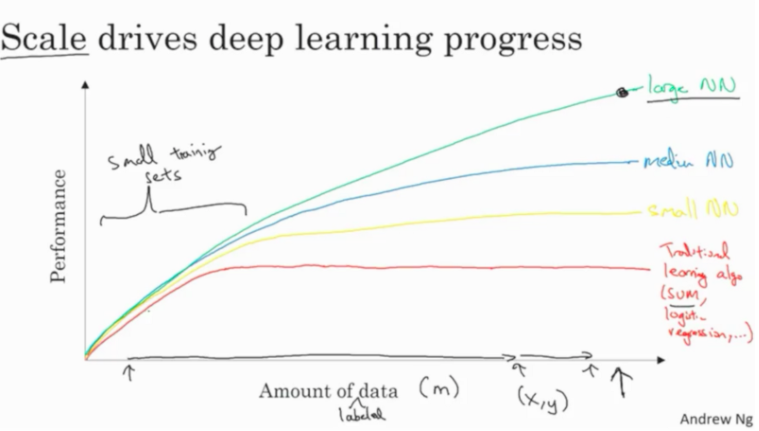
\includegraphics[width=\textwidth]{images/dl_tradeoff.png}
        \end{center}
    \end{column}
    \vline
    \begin{column}{0.5\textwidth}
        \begin{center}
            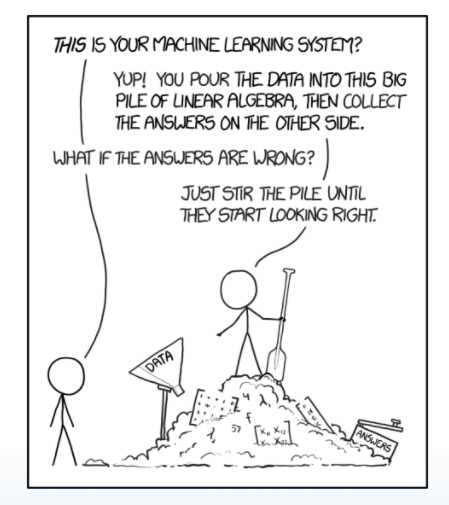
\includegraphics[height=5.5cm]{images/dl_data_joke.png}
        \end{center}
    \end{column}
\end{columns}

\end{frame}
%-------------------------------------------------------------------------------
\begin{frame}
\frametitle{Введение}
\framesubtitle{Проблема данных}

Если мы не знаем паттерна для генерации и хотим уметь обощать, то будем использовать DL и больше данных (Mikolov et al., 2010). \\

\begin{columns}
    \begin{column}{0.5\textwidth}
        Но что делать, есть данных мало?
        \begin{itemize}
            \item Мы не сможем обобщать 
            \item Мы скорее всего переобучимся
            \item При генерации новые сэмплы будут слишком похожи на старые
        \end{itemize}
    \end{column}
    \begin{column}{0.5\textwidth}
        \begin{center}
            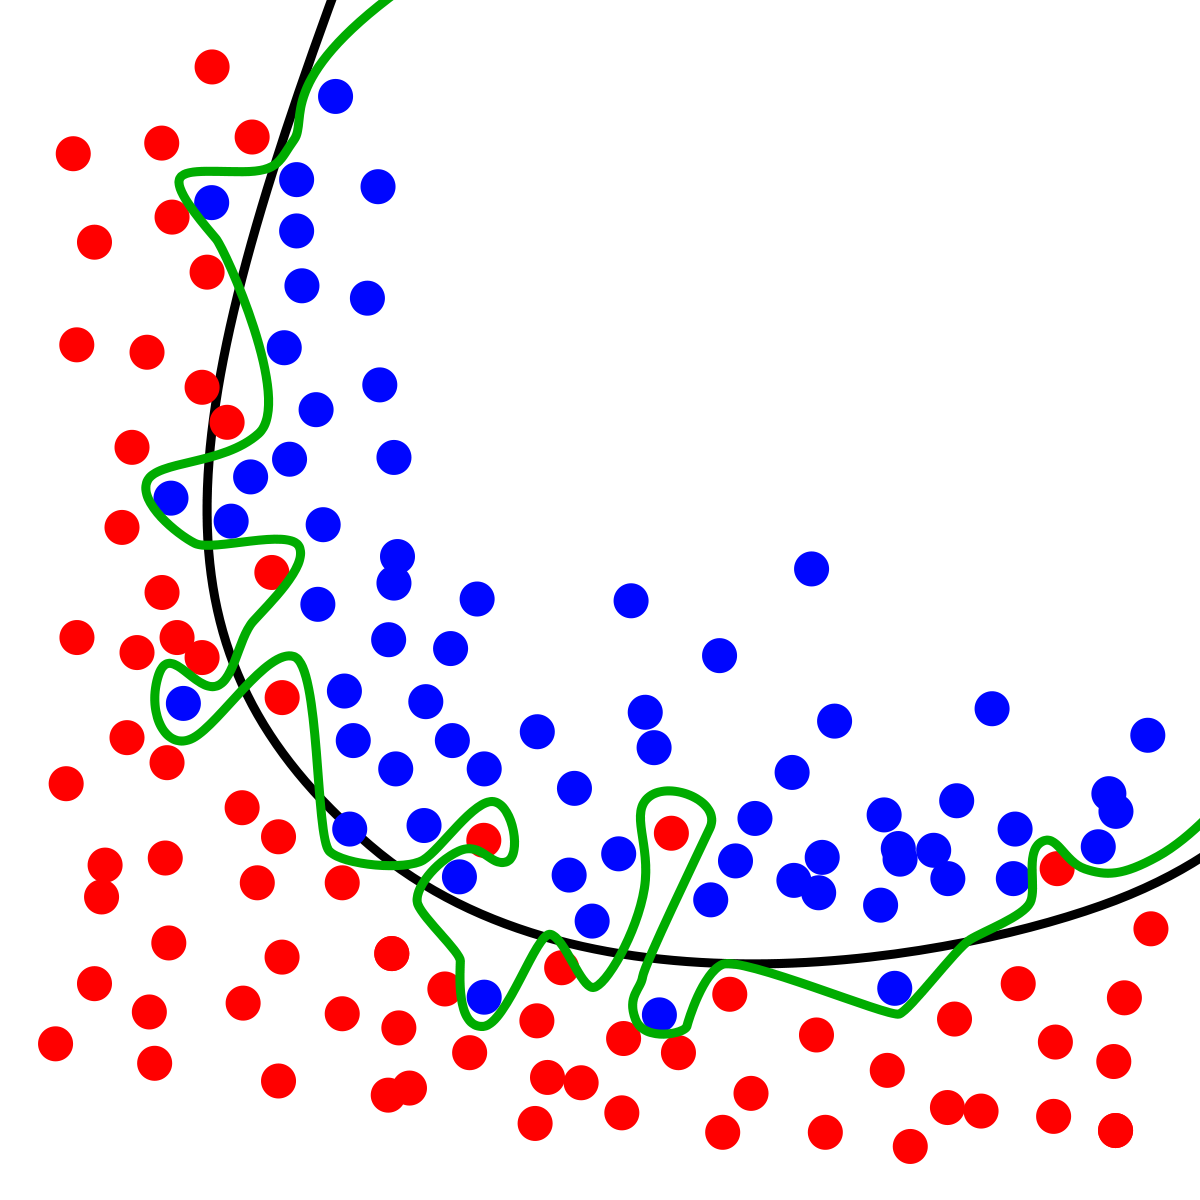
\includegraphics[width=0.7\textwidth]{images/overfitting.png}
        \end{center}
    \end{column}
\end{columns}

\vskip4mm

\underline{Решение}: Искать похожие $X_{\texttt{aux}} \sim X$ in-domain данные из смежных областей.

\end{frame}
%-------------------------------------------------------------------------------
\section{Данные}
\begin{frame}
\frametitle{Данные}
\framesubtitle{Условия задачек}

\begin{columns}
    \begin{column}{0.5\textwidth}
        \begin{itemize}
            \item Разный контекст, форма, требования и сложность
            \begin{itemize}
                \item Сложно выделить шаблон
            \end{itemize}
            \item Собран вручную ($\sim 100$)
            \item Запрос в Stepik
            \begin{itemize}
                \item На английском
                \item С тегами и темами
            \end{itemize}
            \item Расширяемо за счет кравлеров по codeforces и hackerank
        \end{itemize}
    \end{column}
    \begin{column}{0.5\textwidth}
        \begin{columns}
            \begin{column}{0.35\textwidth}
                \begin{center}
                    
\includegraphics[width=\textwidth]{images/stepik.png}
                \end{center}
            \end{column}
            \begin{column}{0.65\textwidth}
                \begin{center}
                    
\includegraphics[width=\textwidth]{images/codeforces.png} \\
                    
\includegraphics[width=\textwidth]{images/hackerank.png}
                \end{center}
            \end{column}
        \end{columns}
    \end{column}
\end{columns}

\vskip3mm

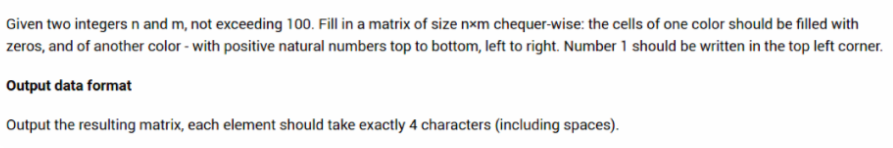
\includegraphics[width=\textwidth]{images/stepik_example.png}

\end{frame}
%-------------------------------------------------------------------------------
\begin{frame}
\frametitle{Данные}
\framesubtitle{Stackoverflow}

\begin{columns}
    \begin{column}{0.65\textwidth}
        \begin{itemize}
            \item Есть готовый за 2008-2016
            \item 2016-2018 получаем с открытого api
            \item Хотя бы с одним тэгом \textit{python}
            \begin{itemize}
                \item Остальные тэги уже проставлены
            \end{itemize}
            \item Замена нод с кодом на $CODE$
            \begin{itemize}
                \item Не портим словарь
                \item Не ищем/учитываем лишние ненужные зависимости
            \end{itemize}
            \item $\Xaux$, но слова и выражения используются в правильном значении
        \end{itemize}
    \end{column}
    \begin{column}{0.35\textwidth}
        \begin{center}
            
\includegraphics[width=0.4\textwidth]{images/stackoverflow.png}
        \end{center}
    \end{column}
\end{columns}

\vskip3mm


\includegraphics[width=\textwidth]{images/stackoverflow_example.png}

\end{frame}
%-------------------------------------------------------------------------------
\begin{frame}
\frametitle{Данные}
\framesubtitle{Docstring}

\begin{columns}[T]
    \begin{column}[T]{0.5\textwidth}
        \begin{itemize}
            \item Кравлер по гитхабу, \textit{python} код
            \item ASCII text без вставок кода + ограничения по длинне
            \item Похожий на английский
            \begin{itemize}
                \item Готовая языковая модель
            \end{itemize}
            \item Тэги
            \begin{itemize}
                \item Entities
                \item Связки сущ. + прилаг.
                \item Top1000
            \end{itemize}
            \item $\Xaux$, но слова и выражения используются в правильном значении
        \end{itemize}
    \end{column}
    \begin{column}[T]{0.5\textwidth}
        \vskip-5mm
        \begin{center}
            Пример
            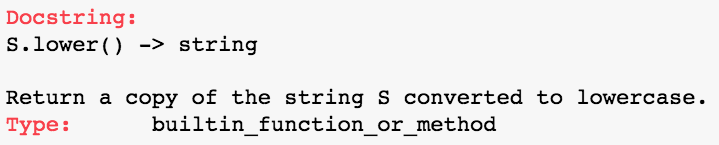
\includegraphics[width=1\textwidth]{images/docstring2.png} \\
            Entities
            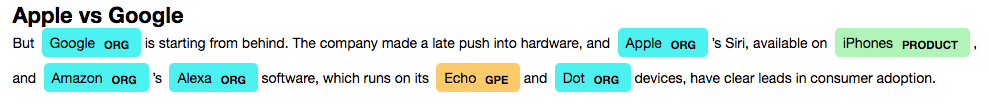
\includegraphics[width=1\textwidth]{images/entities.png} \\
            Дерево разбора
            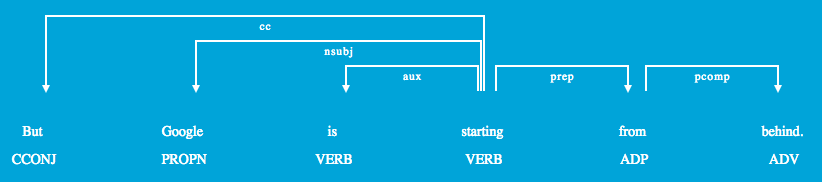
\includegraphics[width=1\textwidth]{images/syntax_tree.png} \\
            Тэги
            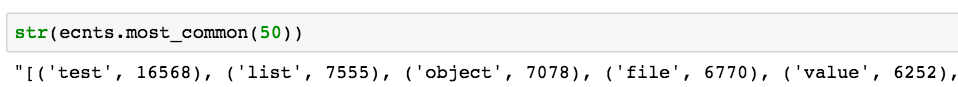
\includegraphics[width=1\textwidth]{images/ecnts.png} \\
        \end{center}
    \end{column}
\end{columns}

\vskip3mm

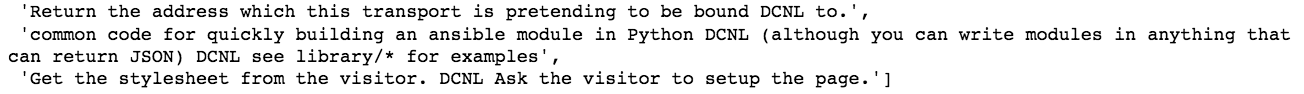
\includegraphics[width=\textwidth]{images/docstring_example.png}

\end{frame}
%-------------------------------------------------------------------------------
\begin{frame}
\frametitle{Данные}
\framesubtitle{Итого}

$$X_{\texttt{data}} = X_1 \cup X_2 \cup X_3$$

\begin{columns}[T]
    \begin{column}[T]{0.33\textwidth}
        \begin{center}
            Условия задачек \\
            \begin{columns}
                \begin{column}{0.35\textwidth}
                    \begin{center}
                        
\includegraphics[width=\textwidth]{images/stepik.png}
                    \end{center}
                \end{column}
                \begin{column}{0.65\textwidth}
                    \begin{center}
                        
\includegraphics[width=\textwidth]{images/codeforces.png} \\
                        
\includegraphics[width=\textwidth]{images/hackerank.png}
                    \end{center}
                \end{column}
            \end{columns}
            \begin{itemize}
                \item $|X_1 \in X| = 5\texttt{k}$
                \item Тэги ($f$) уже проставлены
                \item Собран вручную, но будет готовый
            \end{itemize}
        \end{center}
    \end{column}
    \vline
    \begin{column}[T]{0.33\textwidth}
        \begin{center}
            Stackoverflow \\
            
\includegraphics[width=0.4\textwidth]{images/stackoverflow.png} \\
            \begin{itemize}
                \item Берем вопросы с тэгом \textit{python}
                \item $|X_2 \in X_{aux}| = 600\texttt{k}$
                \item Тэги уже проставлены
                \item Предобработка
            \end{itemize}
        \end{center}
    \end{column}
    \vline
    \begin{column}[T]{0.33\textwidth}
        \begin{center}
            Docstring \\
            \vskip3mm
            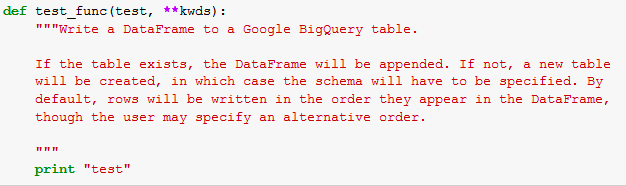
\includegraphics[width=0.9\textwidth]{images/docstring.png} \\
            \vskip3mm
            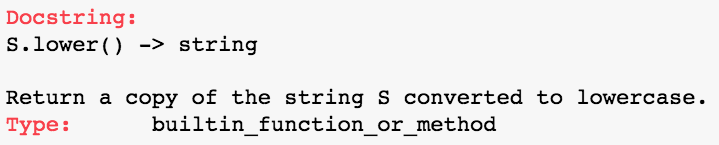
\includegraphics[width=0.9\textwidth]{images/docstring2.png} \\
            \begin{itemize}
                \item $|X_3 \in X_{aux}| = 150\texttt{k}$
                \item Тэги = Entities
                \item Предобработка
            \end{itemize}
        \end{center}
    \end{column}
\end{columns}

\end{frame}
%-------------------------------------------------------------------------------
\section{Генерация}
\begin{frame}
\frametitle{Введение}
\framesubtitle{Изображения vs текст}

\begin{columns}[T]
    \begin{column}[T]{0.5\textwidth}
        \begin{center}
            Изображения \\
            
\includegraphics[width=0.5\textwidth]{images/image_as_func.png} \\
            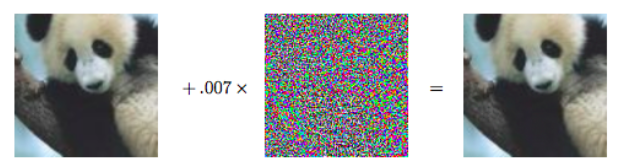
\includegraphics[width=\textwidth]{images/panda_plus_noise.png} \\
            \begin{itemize}
                \item Непрерывное пространство
                \item Набор всевозможных преобразований как дифференцируемых функций
                \item Понятно, куда распространять градиент
            \end{itemize}
        \end{center}
    \end{column}
    \vline
    \begin{column}[T]{0.5\textwidth}
        \begin{center}
            Текст \\
            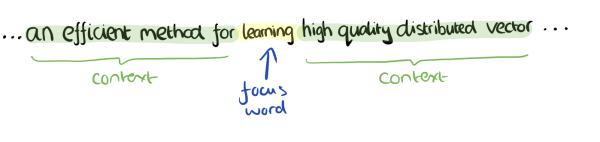
\includegraphics[width=0.9\textwidth]{images/word_context.png} \\
            \begin{itemize}
                \item Дискретное пространство
                \item Переменная длинна
                \item Нет устойчивости к шуму
                \item Long-term зависимости
                \item Омонимия и контекст
            \end{itemize}
        \end{center}
    \end{column}
\end{columns}

\end{frame}
%-------------------------------------------------------------------------------
\begin{frame}
\frametitle{Введение}
\framesubtitle{Генерация текста}

\begin{columns}[T]
    \begin{column}[T]{0.33\textwidth}
        \begin{center}
            RNN \\
            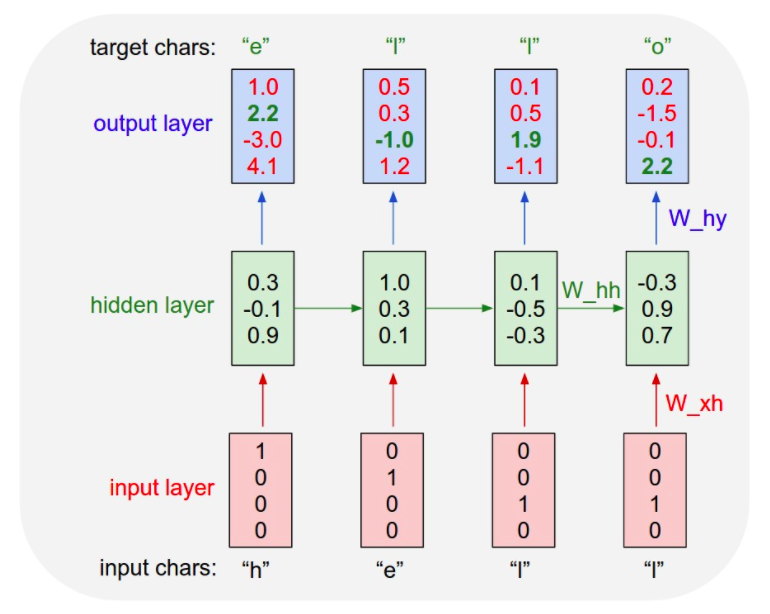
\includegraphics[width=\textwidth]{images/rnn.png} \\
            (Mikolov et al., 2011)
        \end{center}
    \end{column}
    \vline
    \begin{column}[T]{0.33\textwidth}
        \begin{center}
            VAE \\
            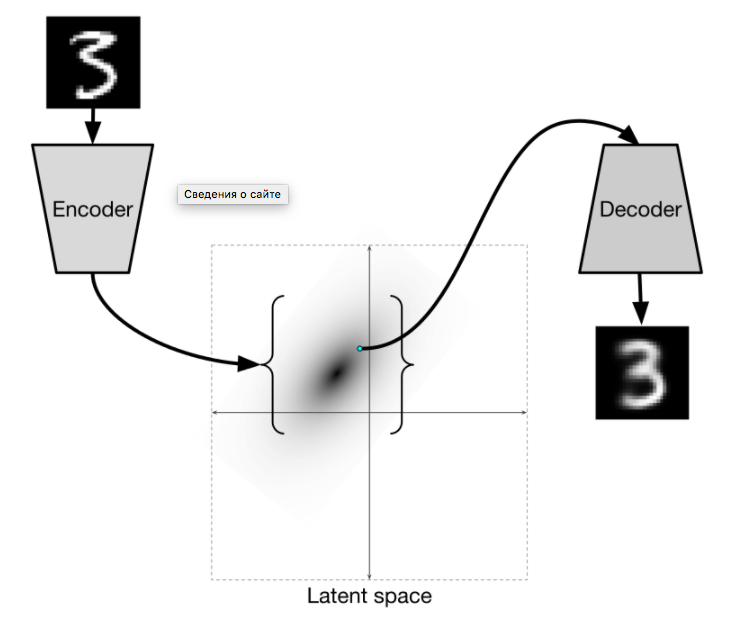
\includegraphics[width=0.9\textwidth]{images/vae.png} \\
            (Bowman et al., 2016; Hu et al., 2018)
        \end{center}
    \end{column}
    \vline
    \begin{column}[T]{0.33\textwidth}
        \begin{center}
            GAN \\
            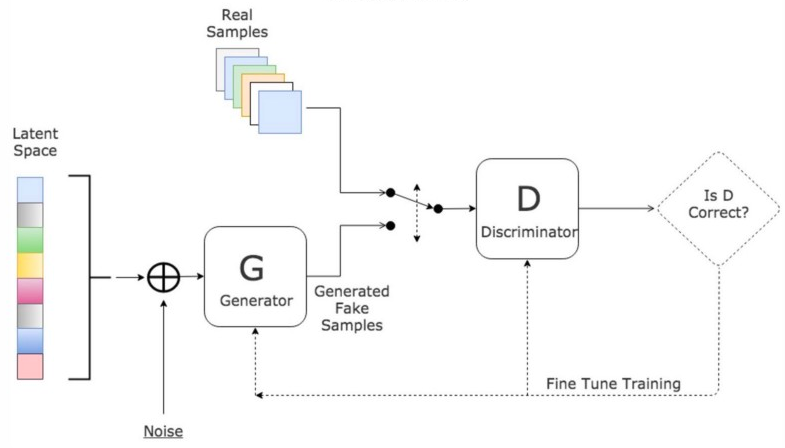
\includegraphics[width=0.9\textwidth]{images/gan.png} \\
            (Yu et al., 2017; Fedus et al., 2018)
        \end{center}
    \end{column}
\end{columns}

\end{frame}
%-------------------------------------------------------------------------------
\section{RNN}
\begin{frame}
\frametitle{RNN}
\framesubtitle{Обзор}

\begin{center}
    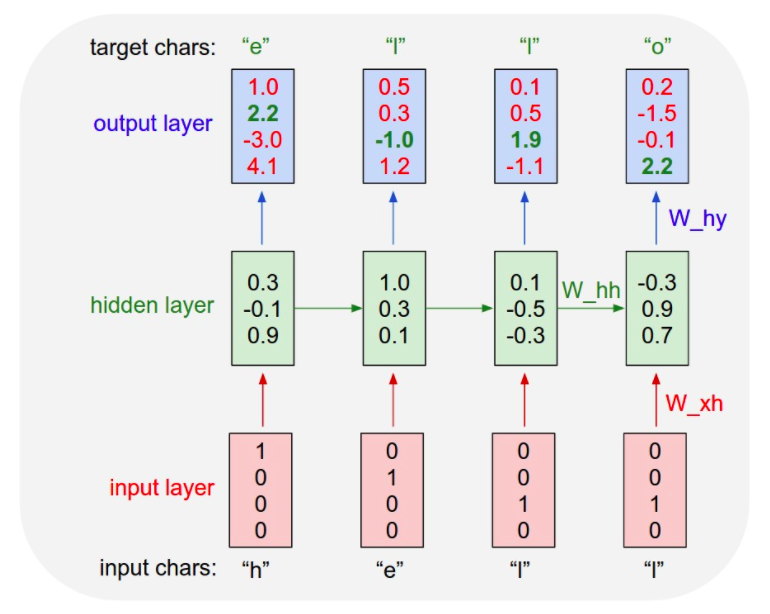
\includegraphics[width=0.65\textwidth]{images/rnn.png}
\end{center}

\end{frame}
%-------------------------------------------------------------------------------
\begin{frame}
\frametitle{RNN}
\framesubtitle{Beam search}

\begin{center}
    $n = 3$ \\
    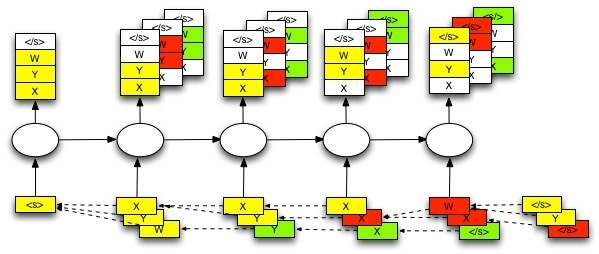
\includegraphics[width=0.95\textwidth]{images/beam_search.jpeg}
\end{center}

\end{frame}
%-------------------------------------------------------------------------------
\begin{frame}
\frametitle{RNN}
\framesubtitle{Seed}

Как задать $RNN$ начальные условия для генерации?
\begin{itemize}
    \item Out-of-band (Chen et al., 2015; Lipton et al., 2015):
    \begin{itemize}
        \item Конкатенация с векторным представлением начальных условий
        \item На каждом шаге/один раз в начале
        \item One-hot/LDA topic modeling/doc2vec
    \end{itemize}
    \item In-band
    \begin{itemize}
        \item Префикс
        \item Префис + суффикс
        $$\texttt{text} \Rightarrow \texttt{tags} + | + \texttt{text} + | + \texttt{tags}$$
        \item Начинаем генерировать с нужного префикса
        \item Отрезаем суффикс
    \end{itemize}
\end{itemize}

\end{frame}
%-------------------------------------------------------------------------------
\begin{frame}
\frametitle{RNN}
\framesubtitle{Реализация}

Модель:
\begin{itemize}
    \item MultiLayerLSTM, 2 слоя
    \item WordRNN/CharRNN/BPERNN
    \item Dropout=0.5 на первом слое
    \item 100 эпох
    \item Out-of-band/In-band
\end{itemize}

\vskip3mm

Результаты:
\begin{itemize}
    \item Долго сходится и плохо интерпретируется
    \item Правдоподобная генерация, но в качестве Seed не получится передать близость к $X$
    \begin{itemize}
        \item Out-of-band учится отделять $X$ от $\Xaux$
        \item In-band путается
    \end{itemize}
\end{itemize}

\end{frame}
%-------------------------------------------------------------------------------
\section{VAE}
\begin{frame}
\frametitle{VAE}
\framesubtitle{Обзор и применение}

\begin{center}
    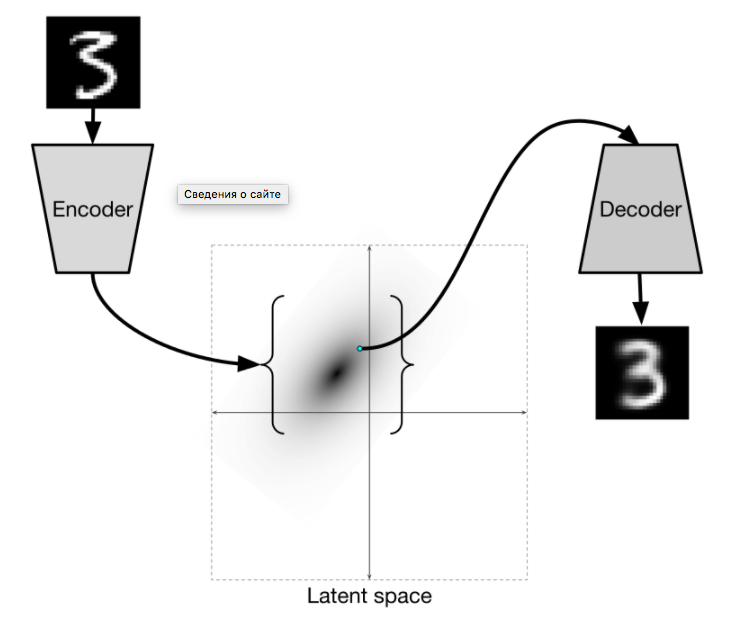
\includegraphics[width=0.65\textwidth]{images/vae.png}
\end{center}

\end{frame}
%-------------------------------------------------------------------------------
\section{GAN}
\begin{frame}
\frametitle{GAN}
\framesubtitle{Обзор и применение}

\TODO{Написать}

\end{frame}
%-------------------------------------------------------------------------------
\section{Оценивание}
\begin{frame}
\frametitle{Оценивание}
\framesubtitle{Метрики}

Как можно оценить результат генерации? (Salimans et al., 16)
\begin{itemize}
    \item Perplexity
    \item Assessors evaluation
        \begin{itemize}
            \item MTurk, Я.Толока
            \item DCG, MAP
        \end{itemize}
    \item Самому
        \begin{itemize}
            \item Generic-генерация
            \item Генерация по заданным темам
        \end{itemize}
\end{itemize}

\end{frame}
%-------------------------------------------------------------------------------
\begin{frame}
\frametitle{Оценивание}
\framesubtitle{Определение perplexity}

$X_{\texttt{train}}, X_{\texttt{test}}$ - разбили датасет $X_{\texttt{data}} \subset X \cup X_{\texttt{aux}}$. \\
Есть языковая модель $M$, обученная на $X_{\texttt{train}}$. Как оценить эффективность? Посчитаем вероятность предложений $W \in X_{\texttt{test}}$.

\begin{block}{Perplexity}
    $PP(W) = P(w_1w_2w_3\dots w_{|W|})^{-\frac{1}{|W|}}$
\end{block}

\begin{block}{Chain rule}
    $PP(W) = \left[\prod\limits_{i=1}^{|W|}{\frac{1}{P(w_i|w_1\dots w_{i-1})}}\right]^{\frac{1}{|W|}}$
\end{block}

\begin{itemize}
    \item Нижний терм в произведении $\Leftrightarrow$ очередной шаг алгоритма
    \item Чем меньше perplexity, тем больше $P(W)$, т.е. тем лучше
    \item Отдельно посчитаем для $X_{\texttt{test}} \cap X$ (это - реально важная метрика)
\end{itemize}

\end{frame}
%-------------------------------------------------------------------------------
\begin{frame}
\frametitle{Оценивание}
\framesubtitle{Таблица perplexity}

\begin{table}
\begin{tabular}{l | l l l l}
\toprule
\textbf{Test} & \textbf{RNN} & \textbf{VAE} & \textbf{CVAE} & \textbf{GAN} \\
\midrule
PTB & 38.93 & \NaN & \NaN & 39.12 \\
CMC & 29.10 & \NaN & \NaN & 29.09 \\
\midrule
$X_{\texttt{test}}$ & 30.29 & \NaN & \NaN & \NaN \\
$X_{\texttt{test}} \cap X$ & 40.10 & \NaN & \NaN & \NaN \\
\bottomrule
\end{tabular}
\caption{Perplexity}
\end{table}

\end{frame}
%-------------------------------------------------------------------------------
\begin{frame}
\frametitle{Оценивание}
\framesubtitle{Примеры}

\begin{center}
    RNN (~20 эпох) \\
    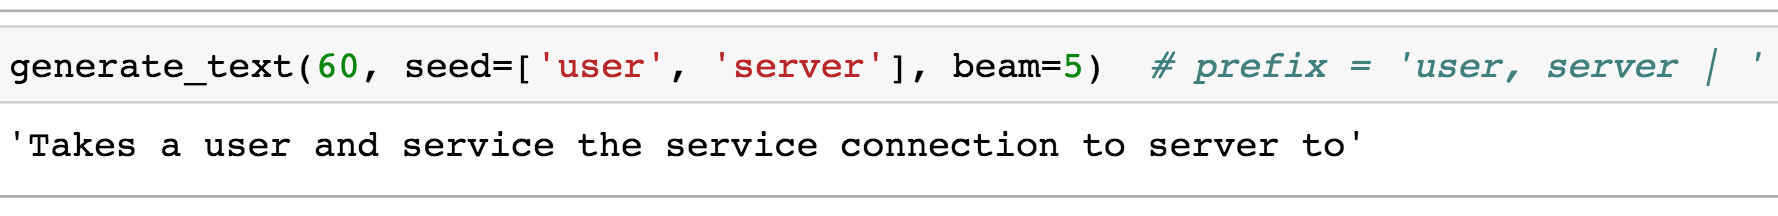
\includegraphics[width=0.8\textwidth]{images/example.png}
\end{center}

% \TODO{Добавить больше}

\end{frame}
%-------------------------------------------------------------------------------
\section{Выводы}
\begin{frame}
\frametitle{Выводы}
\framesubtitle{Результаты}

\begin{itemize}
    \item Анализ state-of-the-art методов генерации текста
        \begin{itemize}
            \item Модификации для наших данных
            \item Сравнение подходов
        \end{itemize}
    \item Анализ влияние данных на генерацию
    \begin{itemize}
        \item Каково влияние $\Xaux$ на генерацию?
        \item Как соотносятся $X$ и $\Xaux$ в терминах латентных представлений?
    \end{itemize}
    \item Метрики и эмпирические проверки, позволяющие оценить сложность задачи
\end{itemize}

% \TODO{Добавить еще}

\end{frame}
%-------------------------------------------------------------------------------
\begin{frame}
\frametitle{Выводы}
\framesubtitle{Будущая работа}

\begin{itemize}
    \item Попытаться проинтерпретировать важной свойств
    \begin{itemize}
        \item Seed для $RNN$
        \item Латентное подпространство для $\Xtest \cap X$ из $VAE$
    \end{itemize}
    \item Больше данных $\Rightarrow$ выделить паттерн для генерации?
    \item Оптимизация скорости для тестирования:
    \begin{itemize}
        \item RNN $\Rightarrow$ CNN
    \end{itemize}
    \item Попробовать GAN'ы
        \begin{itemize}
            \item WC-GAN
            \item SeqGAN
            \item GumbelSoftmax
        \end{itemize}
    \item Генерировать код решения по условию задачи
\end{itemize}

% \TODO{Добавить еще}

\end{frame}
%-------------------------------------------------------------------------------
\section{Ссылки}
\begin{frame}
\frametitle{Ссылки}
\framesubtitle{Статьи, код и контакты}

\begin{enumerate}
    \item \begin{thebibliography}{99}
            \bibitem[Barone, 2017]{p1} Antonio Valerio Miceli Barone (2017)
            \newblock \href{https://arxiv.org/abs/1707.02275v1}{A parallel corpus of Python functions and documentation strings for automated code documentation and code generation}
        \end{thebibliography}
    \item Karpathy, Andrej (2015). \href{http://karpathy.github.io/2015/05/21/rnn-effectiveness/}{“The Unreasonable Effectiveness of Recurrent Neural Networks”.}
    \item \begin{thebibliography}{99}
            \bibitem[Bowman, 2016]{p1} Samuel R. Bowman (2016)
            \newblock \href{https://arxiv.org/abs/1511.06349}{Generating Sentences from a Continuous Space}
        \end{thebibliography}
    \item \begin{thebibliography}{99}
            \bibitem[Hu, 2018]{p1} Zhiting Hu (2018)
            \newblock \href{https://arxiv.org/abs/1703.00955}{Toward Controlled Generation of Text}
        \end{thebibliography}
    \item \begin{thebibliography}{99}
            \bibitem[Wang, 2017]{p1} Heng Wang (2017)
            \newblock \href{https://arxiv.org/abs/1712.00170}{Text Generation Based on Generative Adversarial Nets with Latent Variable}
        \end{thebibliography}
    \item \ULurl{https://github.com/stasbel/task-gen} (Генерация)
    \item \ULurl{https://github.com/stasbel/bachelor-thesis} (Презентация)
    \item \ULurl{https://t.me/stasbel}
\end{enumerate}

\end{frame}
%-------------------------------------------------------------------------------
%	END PRESENTATION SLIDES
%-------------------------------------------------------------------------------
\end{document}